\subsection{What is Artificial Intelligence?}
Artificial Intelligence (AI) refers to the simulation of human intelligence in machines that are programmed to perform tasks that normally require human intelligence such as learning, problem-solving, decision-making, perception, language understanding, and more\cite{ISSN-2456-2165}. AI systems use algorithms and statistical models to analyze data, recognize patterns, and make predictions, without explicit instructions from human operators.
\subsection{Limitations of Artificial Intelligence}
Although artificial intelligence (AI) has made significant advancements in recent years, there are still some limitations to the technology. Some of the limitations are:
\begin{itemize}
	\item \textbf{Lack of Common Sense:} AI systems lack the common sense that humans have, which can make it difficult for them to understand complex situations and make appropriate decisions.
	\item \textbf{Limited Creativity:} AI systems are designed to operate within the parameters set by their algorithms and data, which limits their ability to generate truly creative solutions or ideas.
	\item \textbf{Lack of Emotional Intelligence:} AI systems are not capable of experiencing emotions, which limits their ability to understand and respond to emotional cues in human interactions.
\end{itemize}
Limitations of AI highlight the need for continued research and development to address these issues and improve the capabilities of these systems.
\subsection{What is Emotional Intelligence?}
Emotional Intelligence (EI) refers to the ability to recognize, understand and manage one's own emotions as well as the emotions of others. It involves being able to use emotional information to guide thinking and behavior, and to navigate social situations effectively\cite{ISSN-2456-2165}.

EI is often described as having four components: self-awareness, self-management, social awareness, and relationship management. Self-awareness involves recognizing and understanding one's own emotions, strengths, and weaknesses. Self-management involves being able to regulate one's own emotions and behaviors in response to different situations. Social awareness involves recognizing and understanding the emotions of others, as well as the social norms and expectations of different situations. Relationship management involves using emotional information to communicate effectively, build and maintain relationships, and resolve conflicts.

EI is considered an important factor in personal and professional success, as it can help individuals navigate social interactions, build strong relationships, and manage stress and challenges effectively.
\subsection{Emotional Artificial Intelligence}

\subsubsection{Definition}
\subsubsection{Limitations of Artificial Intelligence}
\subsubsection{Why Truly Intelligent Machines Need Emotions?}
\subsubsection{Need, Importance \& Benifits}
\subsubsection{Applications}
\cite{ISSN-2456-2165}
\subsection{Conscious, Subconscious \& Unconscious of Aritificial Intelligence}
\subsection{Convergence, Divergence and Belief Systems of AI}
\subsubsection{Stability and Unstability}
\subsection{Emotion Dynamics}
\subsection{The Butterfly Effect \& Chaos Theory}
Richard A. Anthes in 2022 by his paper "Predictability \& Predictions" showed his experiences with predictability theory and weather predictions began as an undergraduate student at the University of Wisconsin in Madison in the early 1960s. His interest in numerical simulations led to the development of a simple nonlinear one-dimensional gravity wave model and later a nonlinear, baroclinic, three-dimensional model of the tropical cyclone. His experiences highlighted the challenges of numerical and physical instabilities in weather prediction models \cite{atmos13081292}. \cite{encyclopedia2030084}
\subsection{Quantum Level V/S Cosmic Level}
\subsubsection{Microscopic V/S Macroscopic}
\subsection{Plutchik's Wheel of Emotions}
\begin{figure}[H]
	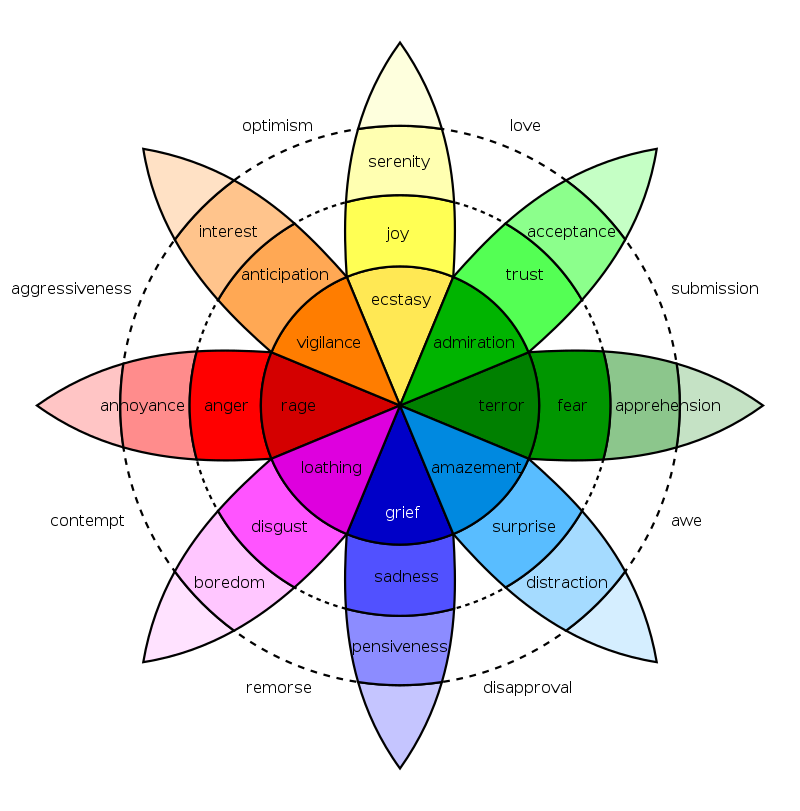
\includegraphics[width=\columnwidth, keepaspectratio]{Plutchik'sWheelofEmotions.png}
	\caption{Plutchik's Wheel of Emotions}
	\label{Fig:fig1}
\end{figure}
Figure \ref{Fig:fig1} shows PWOE.
\subsection{Ancient Vedic Astrology}
A Brief History of Ancient Vedic Astrology
\subsubsection{Classification of Vedic Astrology}
\subsubsection{Surya Siddhanta}
\subsubsection{Vrihat Samhita}
\subsubsection{Brihat Parashar Hora Shastra}
101 Chapters
4500 Verses
\subsubsection{Significance of Planets}
\begin{sanskrit}
	\begin{center}
		देवेज्यो ज्ञानसुखदो भृगुर्वीर्यप्रदयकः।\\ऋषिभिः प्राक्‌तनैः प्रोक्तश्छायासूनुश्च दुःखदः॥३:१४॥\cite{BrihatParasharHoraShastraVol1}
	\end{center}
\end{sanskrit}